\documentclass{beamer}

\usepackage[utf8]{inputenc}
\usepackage[T1]{fontenc}
\usepackage{textcomp}
\usepackage{amsmath, amssymb}
\usepackage{xcolor}
\usepackage{graphicx}
\usepackage{booktabs}
\usepackage{array}
\usepackage{tabularx}
\usepackage{threeparttable}
\usepackage{tikz}
\usepackage{hyperref}

\hypersetup{
  colorlinks=true,
  linkcolor=blue,
  urlcolor=cyan
}

\usetikzlibrary{positioning, arrows.meta}

\usetheme{Boadilla}
\setbeamertemplate{navigation symbols}{}
\setbeamertemplate{footline}[frame number]

\newcommand{\sourceline}[1]{%
  \vspace{0.35em}
  {\tiny \textcolor{gray}{\textit{Source:} #1}}
}

\newcommand{\yenperdollar}{\(\textyen/\$\)}

\title[BOJ and the Yen]{Why Did the Yen Weaken After the Bank of Japan Ended Negative Interest Rates?}
\author[Logan Rechin and Joe White]{Logan Rechin and Joe White}
\institute[Miami University]{Miami University \\ ECO 442}
\date{\today}

\begin{document}

% =========================================================
% TITLE
% =========================================================

\frame{\titlepage}

% =========================================================
% SLIDE 1
% =========================================================

\begin{frame}[t]{Our event}

\begin{itemize}
    \setlength{\itemsep}{0.9em}
    
    \item In March of 2024, the Bank of Japan ended negative interest rates.
    
    \item First rate hike in 17 years.
   
    \item Major shift away from an extremely unusual monetary policy.
    
    \item Normally we would expect the yen to strengthen.
    
    
    \item Instead, the yen weakened.
    
\end{itemize}

\vspace{0.6em}

\textbf{Economic question:} Why did the yen weaken after Japan ended negative rates?

\end{frame}

% =========================================================
% SLIDE 2
% =========================================================

\begin{frame}[t]{What are Negative Interest Rates?}

\begin{itemize}
    \setlength{\itemsep}{0.9em}
    
    \item Negative rates do not mean consumers literally lose cash.
    
    \item Instead, banks can be charged on some reserve balances held at the central bank.
    
    \item Aim is to encourage banks to lend and invest, instead of leaving funds just sitting around.
    
    \item Aggressive form of expansionary monetary policy.
    
\end{itemize}

\vspace{0.6em}

\textbf{Simple idea:} instead of rewarding banks for holding money, the central bank makes holding that money more costly.

\end{frame}

% =========================================================
% SLIDE 3
% =========================================================

\begin{frame}[t]{Example}

\begin{itemize}
    \setlength{\itemsep}{0.8em}
    
    \item A bank keeps \$1{,}000 at the central bank for one year.
    
    \item With a normal interest rate, the bank earns money on that balance.
    
    \item With a negative interest rate, the bank pays to keep that money there instead.
    
\end{itemize}

\vspace{0.6em}

\begin{center}
\begin{tabular}{lcc}
\toprule
 & \textbf{Normal Rate} & \textbf{Negative Rate} \\
\midrule
Initial balance & \$1{,}000 & \$1{,}000 \\
Interest rate & \(+0.5\%\) & \(-0.1\%\) \\
Balance after one year & \$1{,}005 & \$999 \\
\bottomrule
\end{tabular}
\end{center}

\vspace{0.6em}

\begin{center}
\textbf{Normal} \(\rightarrow\) \(+\$5\) \qquad\qquad
\textbf{Negative} \(\rightarrow\) \(-\$1\)
\end{center}

\end{frame}

% =========================================================
% SLIDE 4
% =========================================================

\begin{frame}[t]{Why Did Japan Use Negative Rates?}

\begin{itemize}
    \setlength{\itemsep}{0.9em}
    
    \item Weak inflation, weak demand, and slow growth.
    
    \item Stimulate the economy and move inflation towards the target.
    
    \item Fight stagnation and deflation.
        
    \item Removing negative rates was tied to a long fight against weak price growth.
    
\end{itemize}

\end{frame}

% =========================================================
% SLIDE 5
% =========================================================

\begin{frame}[t]{Why did they end it?}

\begin{itemize}
    \setlength{\itemsep}{0.5em}
    \item Inflation returned (\(\sim 2\%\))
    \item Wages rising strongly
    \item The economy was recovering
    \item Policy had ``fulfilled its role''
\end{itemize}

\vspace{0.4cm}

\begin{center}
    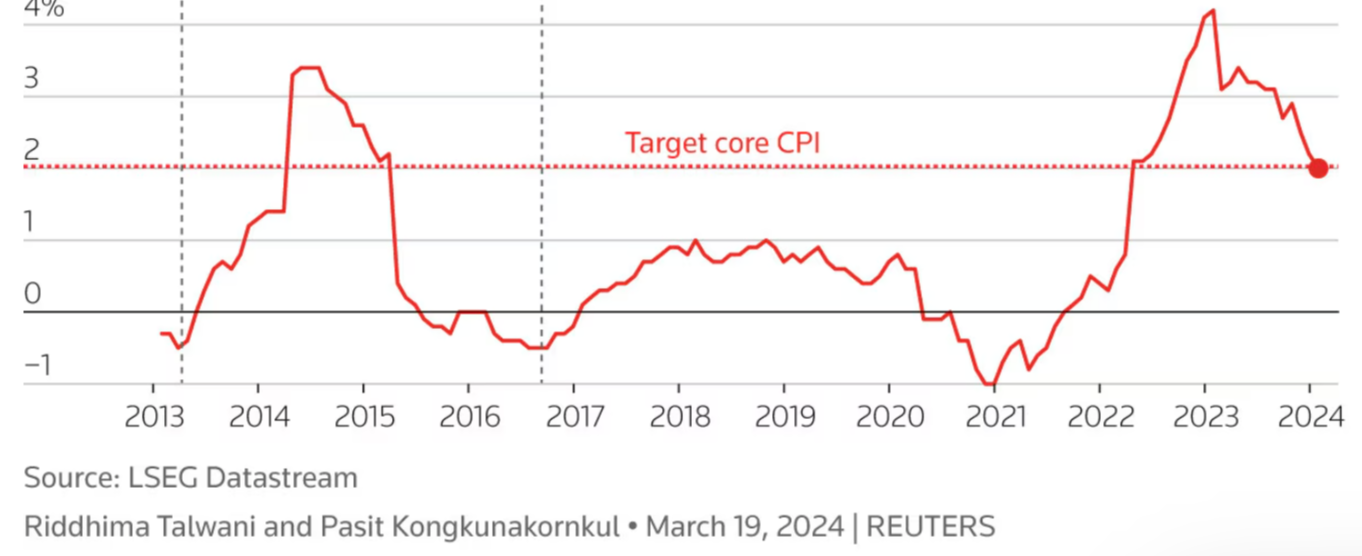
\includegraphics[width=0.78\linewidth]{slide_5_visual.png}
\end{center}

\end{frame}

% =========================================================
% SLIDE 6
% =========================================================

\begin{frame}[t]{What would we expect to see?}

\begin{itemize}
    \setlength{\itemsep}{1.1em}
    
    \item From the asset model, higher Japanese interest rates make Japanese assets more attractive.
    
    \item This shifts the AA curve down.
    
    \item The exchange rate falls, meaning the yen appreciates.
    
\end{itemize}

\centering
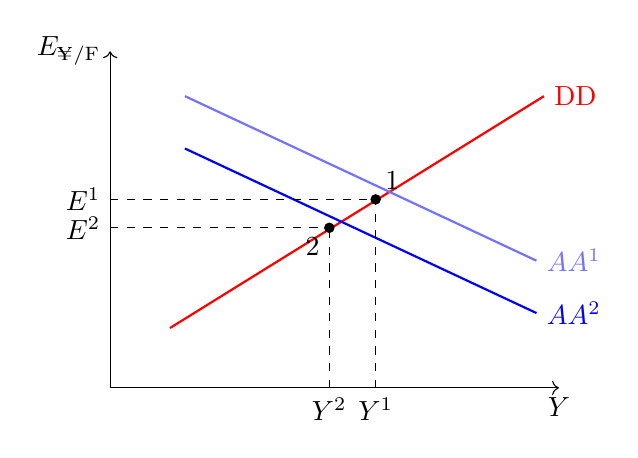
\begin{tikzpicture}[scale=0.95]
    % Axes
    \draw[->] (0,0) -- (0,4.5) node[left] {$E_{\text{\textyen/F}}$};
    \draw[->] (0,0) -- (6,0) node[below] {$Y$};

    % DD
    \draw[thick, red] (0.8,0.8) -- (5.8,3.9) node[right] {DD};

    % AA curves
    \draw[thick, blue!55] (1.0,3.9) -- (5.7,1.7) node[right] {$AA^1$};
    \draw[thick, blue] (1.0,3.2) -- (5.7,1.0) node[right] {$AA^2$};

    % Equilibrium points
    \fill (3.55,2.52) circle (2pt) node[above right] {1};
    \fill (2.93,2.14) circle (2pt) node[below left] {2};

    % Dashed lines
    \draw[dashed] (0,2.52) -- (3.55,2.52);
    \draw[dashed] (3.55,0) -- (3.55,2.52);
    \draw[dashed] (0,2.14) -- (2.93,2.14);
    \draw[dashed] (2.93,0) -- (2.93,2.14);

    % Labels
    \node[left] at (0,2.52) {$E^1$};
    \node[left] at (0,2.14) {$E^2$};
    \node[below] at (3.55,0) {$Y^1$};
    \node[below] at (2.93,0) {$Y^2$};
\end{tikzpicture}

\end{frame}

% =========================================================
% SLIDE 7
% =========================================================

\begin{frame}[t]{What actually happened and why?}

\begin{itemize}
    \setlength{\itemsep}{0.5em}
    \item After the BOJ ended negative rates, the yen weakened rather than strengthened.
    
    \item The BOJ’s move was small and U.S. and other foreign interest rates were still much higher, so investors continued to prefer foreign assets.
\end{itemize}

\vspace{0.25cm}

\begin{center}
    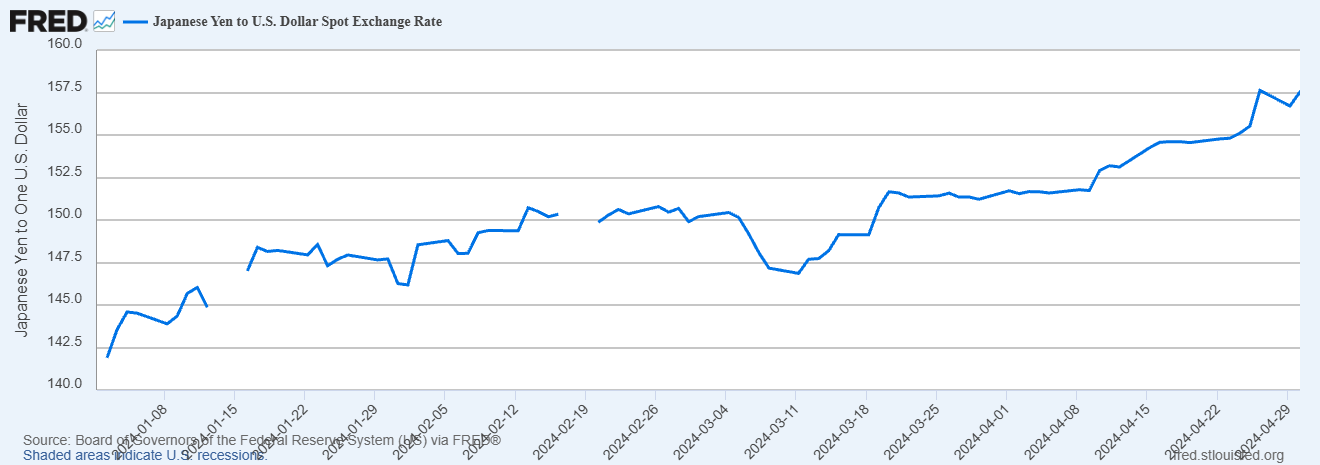
\includegraphics[width=0.76\linewidth]{project_6_graph.png}
\end{center}

\end{frame}

% =========================================================
% SLIDE 8
% =========================================================

\begin{frame}[t]{What does a weaker yen mean?}

\begin{itemize}
    \setlength{\itemsep}{0.55em}
    \item A weaker yen makes Japanese exports cheaper to foreign buyers, helping exporters and making Japan a good destination for tourists.
    \item It also makes imports more expensive in Japan, raising the cost of foreign goods and putting upward pressure on domestic prices.
\end{itemize}

\vspace{0.2cm}

\begin{center}    
    \vspace{0.15cm}
    
    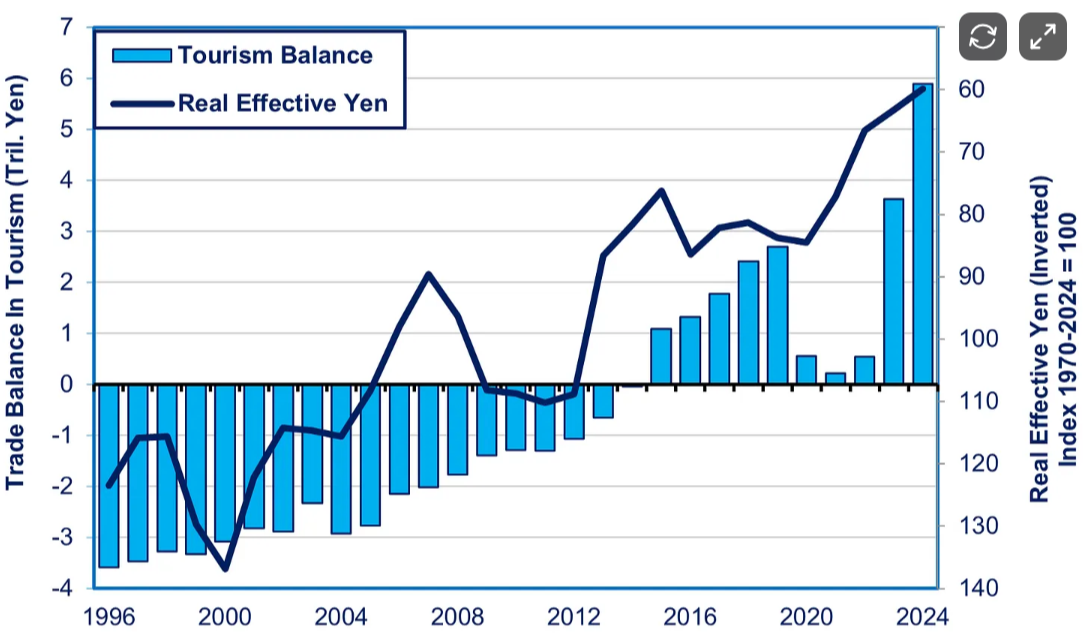
\includegraphics[width=0.76\linewidth]{tourism.png}
\end{center}

\vspace{0.2cm}

{\small Katz, \textit{The Weak Yen Reflects Weak Japan} (2025)}

\end{frame}

% =========================================================
% SLIDE 9 / CONCLUSION
% =========================================================

\begin{frame}[t]{Conclusion}

\begin{itemize}
    \setlength{\itemsep}{0.6em}
    \item Japan ended negative interest rates, but the yen weakened instead of strengthening.
    \item The BOJ's move was small, while U.S. and foreign interest rates remained much higher.
    \item As a result, investors still saw dollar and other foreign assets as more attractive.
    \item This shows that exchange rates depend on relative returns and expectations, not just the policy headline.
\end{itemize}

\end{frame}

% =========================================================
% FINAL SLIDE
% =========================================================

\begin{frame}{Thank you}
\centering
\Large Questions?
\end{frame}

% =========================================================
% APPENDIX / SOURCES
% =========================================================

\appendix
\setbeamertemplate{footline}{}

\begin{frame}[allowframebreaks]{Sources}
\small
\begin{itemize}
    \setlength{\itemsep}{0.8em}

    \item Board of Governors of the Federal Reserve System (US), \textit{Japanese Yen to U.S. Dollar Spot Exchange Rate} [DEXJPUS], retrieved from FRED, Federal Reserve Bank of St. Louis. \\
    \url{https://fred.stlouisfed.org/series/DEXJPUS}

    \item Katz, Richard, \textit{The Weak Yen Reflects Weak Japan}. \\
    \url{https://richardkatz.substack.com/p/the-weak-yen-reflects-weak-japan}

    \item Feingold, Spencer, World Economic Forum, \textit{Japan ends negative interest rates economy monetary policy}. \\
    \url{https://www.weforum.org/stories/2024/03/japan-ends-negative-interest-rates-economy-monetary-policy/}

    \item CNBC, \textit{Bank of Japan March 2024 policy decision}. \\
    \url{https://www.cnbc.com/2024/03/19/bank-of-japan-boj-march-2024-policy-decision-mpm-meeting.html}

\end{itemize}
\end{frame}

\end{document}
